%----------------------------------------
% Write your notes here
%----------------------------------------

\section{Simpson's Paradox}
Selection bias can be so large that observational and causal estimates give opposite effects (e.g., going to hospitals makes you less healthy)
\subsection{Comparing old vs. new algorithm}
Two algorithms, A (production) and B (new) are running on the system. From the system logs, data is collected for 1000 sessions for each algorithm. Measure CTR. Which algorithm is better?
  \begin{center}
      \begin{tabular}{ | l | l |}
      \hline
      Old Algorithm (A) & New Algorithm (B)\\ \hline
      50/1000(5\%) & 54/1000(5.4\%) \\ \hline
      \end{tabular}
  \end{center}
Frequent users of the Store tend to be different from new users. So lets look at CTR separately. The Simpson's paradox: 
  \begin{center}
      \begin{tabular}{ | l | l |l |}
      \hline
      CTR & Old Algorithm (A) & New Algorithm (B)\\ \hline
      CTR for Low-Activity users & 10/400(2.5\%) & 4/200(2\%) \\ \hline
      CTR for High-Activity users & 40/600(5\%) & 50/800(6.2\%) \\ \hline
      Total CTR & 50/1000(5\%) & 54/1000(5.4\%) \\ \hline
      \end{tabular}
  \end{center}
Is Algorithm A better? Answer (as usual): may be, may be not. Algorithm A could have been shown at different times than B. You could have also targeted it to people with high activity. There are also much more people in the new algorithm. Essentially, you can play around and find different algorithms that work well. There are many other hidden casual variations, like income level and stratification (we think that the thing we are changing will have different effects on different groups).

\subsection{Example: Simpson's paradox in Reddit}
If you look at the average number of words on Reddit and condition on different years you will notice that it is decreasing over time. That is, the average comment length is decreasing over time, which could be a worrying sign if you are Reddit. This would mean that Reddit would need to find ways to make people write more. However, if you condition on when a person joined Reddit you will find that the number of comments increases over time. For some reason people who join later seem to comment less and the early adopters of Reddit are the most active. Now Reddit's problem changes. They don't want people to write more, what they want is to attract more of those "good" people.

\section{Counterfactuals}
To isolate the causal effect, we have to change one and only one thing (hospitals visits), and compare outcomes. That is, in an ideal world we would take the world and make a clone world. In one case we would bring the guy to the hospital and in the other case we wouldn't. The only thing that differs between the two cases is whether or not we brought the guy to the hospital, everything else is the same. This is the core idea of what we try to do in an experiment. However, in practice it hard to do an experiment and say that world 1 and world 2 are equal except for the thing that we changed.

\begin{figure}[ht]
  \begin{center}
    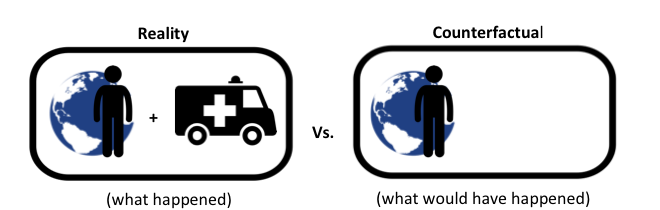
\includegraphics[width=0.5\textwidth]{figures/counterfactuals.png}
  \end{center}
\end{figure}

\section{Random assignment}
We can use randomization to create two groups that differ only in which treatment they receive, restoring symmetry. For each person, we will flip a coin and randomly assign them to going to the hospital or not going to the hospital. There are going to be healthy and sick people in each group. On average the people who get sent and not sent to the hospital is the same, i.e. those groups should be identical because nothing else affected whether or not they went to the hospital. We can then measure the effect of people getting treated at hospitals or not. 

\begin{figure}[ht]
  \begin{center}
    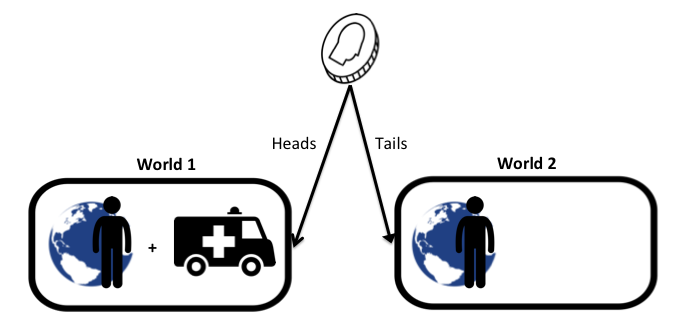
\includegraphics[width=0.5\textwidth]{figures/random_assignment.png}
  \end{center}
\end{figure}

Random assignment determines the treatment independent of any confounds.
\begin{figure}[ht]
  \begin{center}
    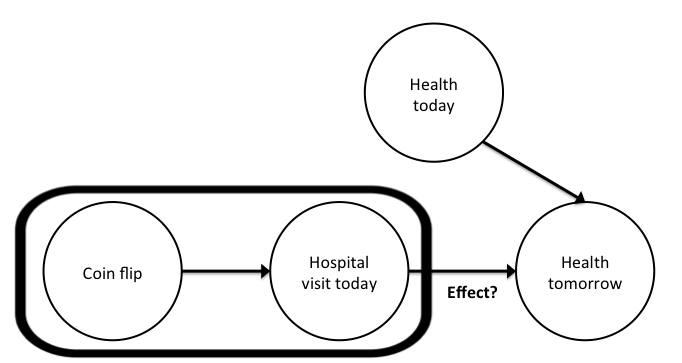
\includegraphics[width=0.5\textwidth]{figures/random_assignment_2.png}
  \end{center}
\end{figure}

\section{Basic identity of causal inference}
The observed difference is now the causal effect: Observed difference = Causal effect - Selection bias = Causal effect
\\ Selection bias is zero, since there's no difference, on average between those who were hospitalized and those who weren't.

\section{Experiments}
\subsection{Caveats/limitations}
Random assignment is the "gold standard" for causal inference, but it has some limitations:
\begin{itemize}
  \item Randomization often isn't feasible and/or ethical (often happens in medical settings)
  \item Experiments are costly in terms of time and money
  \item It's difficult to create convincing parallel worlds
  \item Inevitably people deviate from their random assignments
\end{itemize}
\subsection{Two goals for experiments}
\begin{enumerate}
  \item Internal validity: Could anything other than the treatment (i.e. a confound) have produced this outcome?
  	\begin{itemize}
  		\item Did doctors give the experimental drug to some especially sick patients (breaking randomization) hoping that it would save them?
	\end{itemize}
  \item External validity (Generalization): Do the results of the experiment hold in settings we care about?
  	\begin{itemize}
  		\item Would this medication be just as effective outside of a clinical trial, when usage is less rigorously monitored?
	\end{itemize}
\end{enumerate}
\subsection{How we conduct behavioral experiments and write academic papers across the social sciences
}
\begin{enumerate}
  \item Lab Experiment - what are held at colleges
  	\begin{itemize}
  		\item Better internal validity (correctness): Greatest procedural control, can carefully curate situations
        \item But less external validity (generalization): Artificial context, simple tasks, demand effects, homogeneous (WEIRD - Western Educated Industrialized Rich Democratic) subject pools, time/ scale limitation - You can’t keep people there and you can only bring in a certain number of people
	\end{itemize}
  \item Field Experiment - run an experiment in the real world
  	\begin{itemize}
  		\item Better generalization: Experiment findings apply to at least one real-world setting
        \item But: Less control, more potential confounds, demand of experiment conflict with goals of real organizations, more effort to conduct and manage, more room for error
	\end{itemize}
\end{enumerate}
These kinds of issues also come up in systems as well. Even in the systems that we build ourselves it is not that simple. Internal validity is a problem at companies like Microsoft and Google. If your system has an A/B test you should wait at least 6 months because there are so many things that happen before your code reaches the user. Generalization also comes in. Suppose you run your code and it works well in New York, will it also work well in another city, in another country?

\subsection{Natural experiments}
Sometimes we get luck and nature effectively runs experiments for us e.g:
	\begin{itemize}
    	\item As-if random: People are randomly exposed to water sources
        \item Instrumental variables: A lottery influences military service
        	\begin{itemize}
            	\item Idea: An instrument independently shifts the distribution of a treatment
            \end{itemize}
        \item Discontinuities: Star ratings get arbitrarily rounded
        \item Difference in differences: Minimum wage changes in just one state
    \end{itemize}
\subsection{Behavioral science labs are very limiting}
Pros: 
	\begin{itemize}
		\item High degree of procedural control, Optimized for causal inference
	\end{itemize}
Cons (limitations):
	\begin{itemize}
		\item Artificial environment, Simple tasks, demand effects, Homogeneous (WEIRD) subject pools, Time/scale limitations, Expensive, difficult to set up
	\end{itemize}


\subsection{Experiments are underpowered}
Two-thirds of psychology studies don't replicate! This shows how hard it is to do experiments properly. And if you do do it properly you should be able to run the experiment again and get the same results.

\subsection{Most social science experiments aren't social}
The vast majority of experiments are done with individuals as it is harder to do experiments on groups of people. Therefore, experiments are focused on individual behavior: logistically it's just easier. We actually don't know the causal effects of policies in many large-scale, collective behavior settings. Some examples include: economic inequality, systems of governance, and the black box of macroeconomic policy.

\subsection{So, about them experiments}
They are costly run but are limited in the types of questions they can answer. Large-scale observational data is useful for building predictive models of a static world. Randomized experiments are like custom-made datasets to answer a specific question. Moreover, published experimental research is probably wrong and they are far from answering many big important questions. So how do we fix this? By expanding the experiment design space.

\begin{figure}[ht]
  \begin{center}
    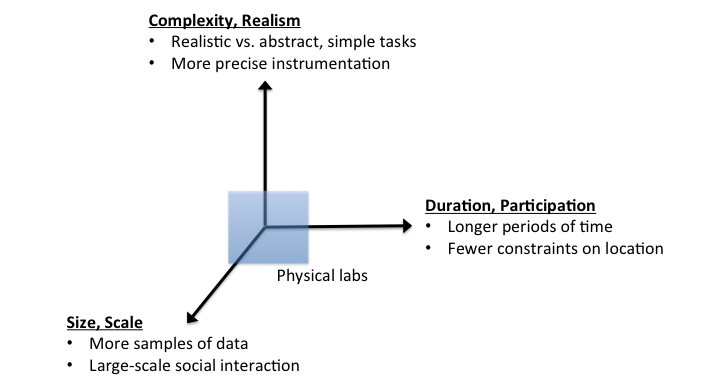
\includegraphics[width=0.5\textwidth]{figures/expanding_experiment.png}
  \end{center}
\end{figure}
